\documentclass[12pt]{article}

% PACKAGES
\usepackage[ngerman]{babel}
\usepackage{lmodern} % Schriftart
\usepackage{bookmark} % Für PDF Lesezeichen
\usepackage{caption} % Für \caption*{}
\usepackage{siunitx} % SI-Einheiten
\usepackage{mathtools} % Verbessertes "amsmath" (https://de.overleaf.com/learn/latex/Articles%2FMathtools_-_for_beautiful_math)
\usepackage{xcolor}   % Farbiger Text (https://www.overleaf.com/learn/latex/Using_colours_in_LaTeX)
\usepackage{geometry} % Zur Einstellung des Layouts
\usepackage{titlesec} % Einteilung des Inhalts (https://de.overleaf.com/learn/latex/Sections_and_chapters)
\usepackage{fancyhdr} % Für Kopf-/ und Fußzeilen (https://www.overleaf.com/learn/latex/Headers_and_footers)
\usepackage{parskip} % Änderung von Absätzen und Absatzeinzügen
\usepackage{biblatex} % Verweise und Referenzen
\usepackage{float} % Benötogt für Figuren und Tabellen
\usepackage{graphicx} % Platzhalter Bilder
\usepackage{booktabs} % Tabellen 
\usepackage{csquotes} % Recommended package for biblatex
\usepackage{hyphenat}
\usepackage{listings} % for typesetting code 
\usepackage{graphicx}
\usepackage{caption}
\usepackage{subcaption}
\usepackage[version=4]{mhchem}
\usepackage{amsfonts}
\usepackage{makecell}
% SETUP 
\setlength{\headheight}{15.059pt} % Set headheight to at least 14.5pt
\addtolength{\topmargin}{-2.5pt} % Make topmargin smaller to compensate
\sisetup{
  output-decimal-marker={,},
  per-mode=fraction,
  fraction-function=\tfrac,
  separate-uncertainty=true
}

\addbibresource{Ressourcen/V61.bib}
\geometry{ %A4
  a4paper,
  total = {170mm,240mm},
  left = 20mm,
  top = 30mm
}
\pagestyle{fancy}
\captionsetup[figure]{
    justification=centering, % Centered captions
    labelsep=colon, % Separate label and caption with a period
    singlelinecheck=false, % Always center even if the caption is short
    labelfont=bf % Bold captions
}
% COMMANDS
\newcommand{\uproman}[1]{\uppercase\expandafter{\romannumeral#1}} % Römische Zahlen

\sisetup{
  per-mode=fraction,
  fraction-function=\tfrac,
  separate-uncertainty=true,
  output-decimal-marker={,}
}
% DOC
\begin{document}

% HEADER
\begin{titlepage}
    \centering
    \vspace*{1cm}
    \includegraphics[width=0.5\textwidth]{Ressourcen/tud_logo_schwarz(RGB)}\\
    \vspace*{0.25cm}
    \large\textmd{Fakultät Physik} \\
    \vspace*{6cm}
    \huge \bfseries FP-2024 - Versuch V18\\
    \vspace*{0.25cm}
    \large Germaniumdetektor\\
    \vspace*{0.25cm}
    \large\textmd{\href{mailto:jan.oppoli@tu-dortmund.de}{Jan Oppoli}} \\
    \vfill
    \small\textmd{Versuch durchgeführt am 24. Juni 2024}\\
    \small\textmd{Abgabe erstellt am \today}
  \end{titlepage}
  \tableofcontents 
  \newpage
\newpage

\section{Zielsetzung}\label{sec:zielsetzung}
Ziel des vorliegenden Versuchs ist es, mithilfe eines hochreinen Germaniumdetektors verschiedene Radioaktive Gammastrahler auf ihre Charakteristika, wie die Vollenergienachweiswahrscheinlichkeit, zu untersuchen.
Nach einer Energiekalibration mittels hinreichend dokumentierter Probe werden die Spektren von sowohl bekannten Materialien, als auch zu bestimmenden Elementen gemessen und ausgewertet.
Aufgrund des hohen Energieauflösevermögens sind Germaniumdetektoren von enormem Wert für die Gamma-Spektroskopie.
\section{Theorie}\label{sec:theorie}
Nachdem zunächst auf den Grundlegenden Aufbau eines Lasers und die Einzelheiten des Entstehungsprozesses von Laserstrahlung und relevante charakteristische Eigenschaften der Wellen eingegangen wird, folgt mit diesem Wissen eine Einführung in die Funktionsweise des verwendeten \ce{He}-\ce{Ne}-Lasers.
\subsection{Aufbau eines Lasers}
Im wesentlichen besteht ein Laser aus drei Komponenten: dem \textbf{aktiven Medium}, der (selektiven) \textbf{Energiepumpe} und dem \textbf{Resonator}.\\
Das Aktive Medium ist ein Material, welches unter speziellen Vorraussetzungen die Fähigkeit besitzt, die Intensität von durchlaufendem Licht zu verstärken. Dies geschieht, da Atome in solchen Konfigurationen angeregt werden, die induzierte Emission von Photonen wahrscheinlicher als Absorption für bestimmte Frequenzen werden lassen(siehe \hyperref[subsec:entstehung]{Entstehung von Laserstrahlung}).\\
Die Energiepumpe liefert die nötige Energie um die Atome in die gewünschten angeregten Zustände zu heben. Erst durch sie kann der Laserbetrieb ermöglicht werden.\\
Der Resonator, typischerweise bestehend aus zwei Spiegeln, sorgt dafür, dass das Licht mehrmals das aktive Medium durchläuft indem er es hin- und herreflektiert. So kann die Verstärkung der Intensität signifikant genutzt werden, um einen stabilen Strahl zu konstruieren. Diese Energie des Laserstrahls wird zu einem großen Teil im Resonator in wenigen Resonatormoden gespeichert, was zu einer hohen Strahlungsdichte in ausgewählten Wellenlängen führt.\cite{Demtroeder} 
\subsection{Entstehung von Laserstrahlung}\label{subsec:entstehung}
Durch die dem System mittels der Pumpe hinzugeführte Energie werden die Atome des aktiven Mediums von ihrem Grundzustand in verschiedene höher gelegene Energieniveaus gehoben.
Sei etwa $k$ ein energetisch höherer quantenmechanischer Zustand des Atoms als ein mit ihm durch einen erlaubten Übergang verbundener Zustand $i$, so würde im thermischen Gleichgewicht für die Besetzungszahlen der Zustände $N_i>N_k$ gelten. Die erwähnte selektive Energiezufuhr führt nun dazu, dass wie in \autoref{fig:inversion} dargestellt, sich die Besetzungsverteilung verändert, es tritt \textbf{Besetzungsinversion} auf.
\begin{figure}[H]
    \centering
    \includegraphics[scale=0.5]{Ressourcen/inversion.png}
    \caption{Thermische Besetzungsverteilung (durchgezogen) und Inversion (gestrichelt)\cite{Demtroeder}}\label{fig:inversion}
\end{figure}
Trifft ein Photon der Frequenz $\nu = \frac{E_k-E_i}{h}$ auf ein angeregtes Atom oder Molekül der Energie $E_k$, so kann es dieses dazu veranlassen in den tieferen Zustand $E_i$ überzugehen unter Emission eines Photons derselben Frequenz und Richtung.

\subsection{Eigenschaften von Laserstrahlung}
\subsection{Funktionsweise eines He-NeLasers}
\section{Aufbau}\label{sec:aufbau}
Wie in \autoref{fig:aufbau} zu sehen, besteht der Versuchsaufbau aus einem Laserrohr, welches mit dem aktiven Medium, einem \ce{He}-\ce{Ne}-Gasgemisch gefüllt ist, dem Resonator in Form von zwei Spiegeln und einem Justierlaser mit der Wellenlänge $\lambda=\SI{523}{\nano\meter}$ inklusive Blende zur Justage des Hauptlasers. Alle Komponenten sind mithilfe von Reitern auf einer Schiene platziert, um kontrollierte Abstandskonfigurationen zu ermöglichen.

\begin{figure}[H]
    \centering
    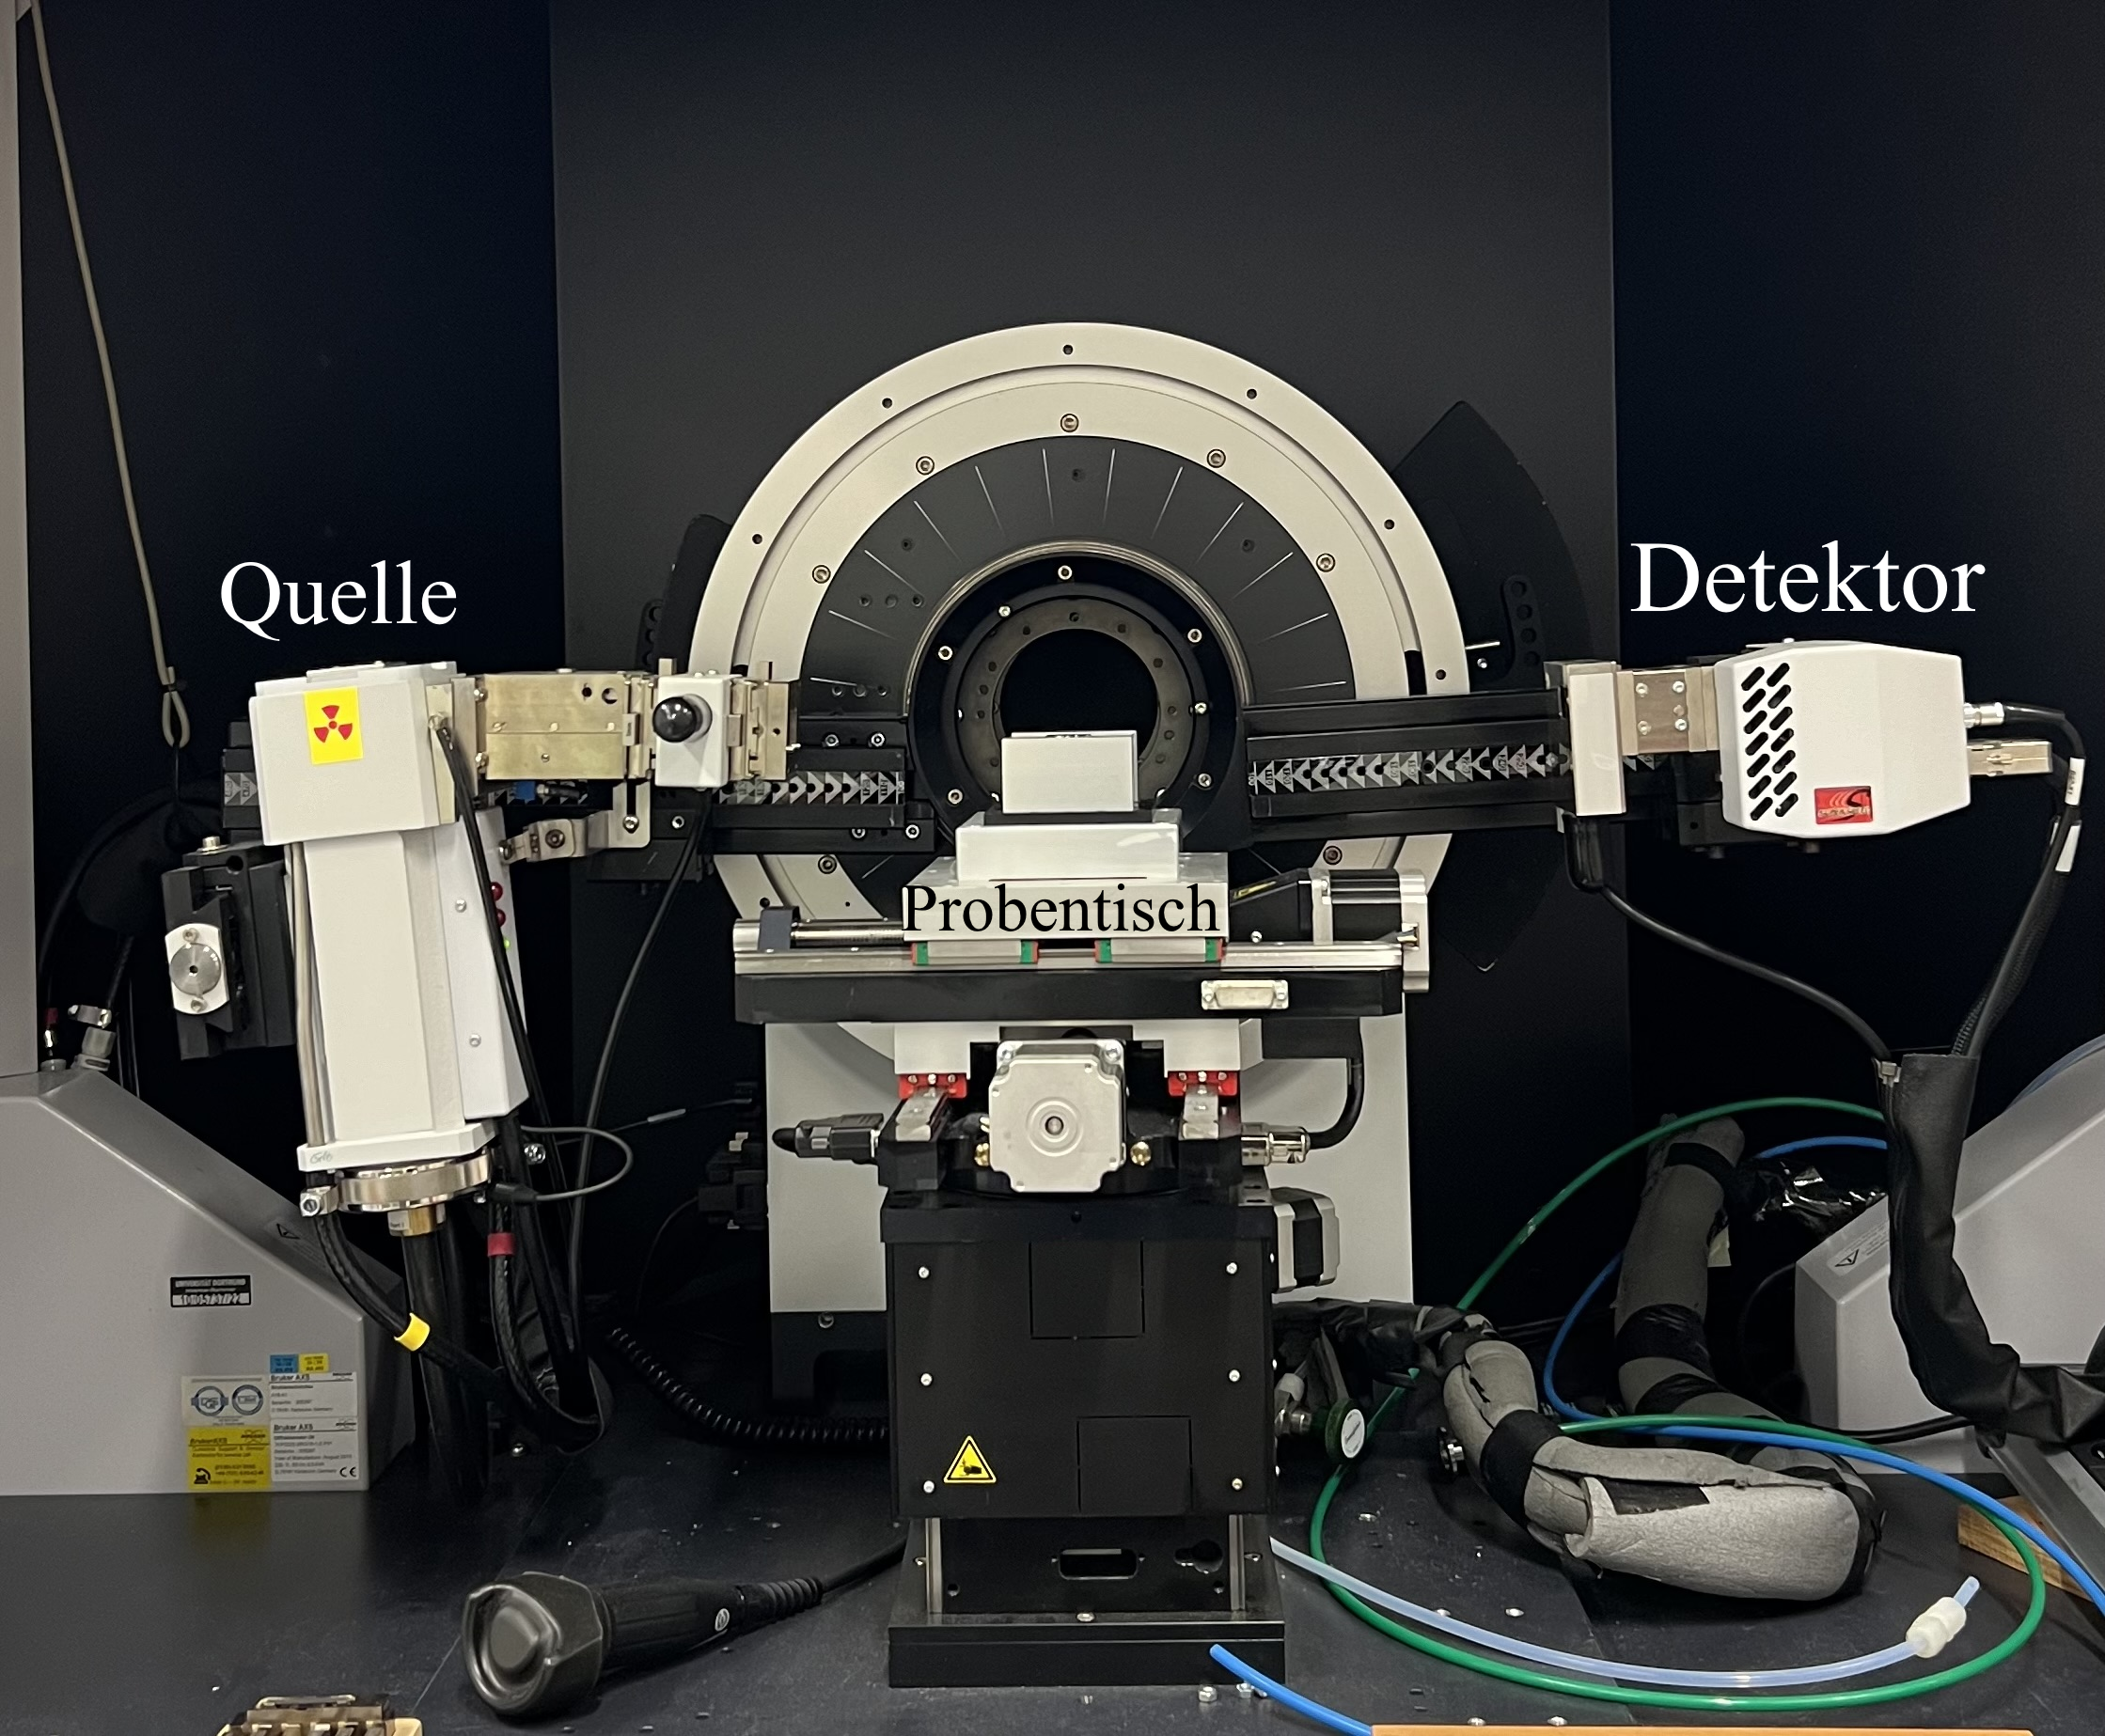
\includegraphics[scale=0.5]{Ressourcen/aufbau.png}
    \caption{Komponenten und Komposition des Verwendeten \ce{He}-\ce{Ne}-Lasers\cite{anleitung}}\label{fig:aufbau}
\end{figure}

\subsection{Laserrohr und Resonator}
Im Laserrohr der Länge $l=\SI{408}{\centi\meter}$ und des Durchmessers $d = \SI{1.1}{\milli\meter}$ bilden Elektroden die Energiepumpe, um für eine Inversion des Gasgemischs zu sorgen und die Enden sind mit Brewsterfenstern zur Selektion einer Polarisationsrichtung versehen. Am Laserrohr sowie den Resonatorspiegeln befinden sich Justierschrauben, welche die Ausrichtung und somit die stabile Funktion des Lasers ermöglichen.

\subsection{Spiegel}
Die zur Verfügung stehenden Spiegel können \autoref{tab:spiegel} entnommen werden.

\begin{table}[H]
  \centering
  \caption{Mögliche Spiegel im Versuchsaufbau und Eigenschaften dieser\cite{anleitung}}
  \begin{tabular}{c | c | c}
    \toprule
    Spiegel & Bezeichnung & Oberflächenbeschaffenheit \\
    \midrule
    plan    & flat/flat            & HR (high reflectivity) R $\geq 99\%$ \\
    konkav  & r=1000 mm/flat       & HR (high reflectivity) R $\geq 99\%$ \\
    konkav  & r=1400 mm/flat       & HR (high reflectivity) R $\geq 99\%$ \\
    konkav  & r=1400 mm/flat       & OC (out coupling) T=1.5,\dots 1.8\% \\
    \bottomrule
  \end{tabular}
  \label{tab:spiegel}
\end{table}

\subsection{Messkomponenten}
Zusätzlich werden verschiedene Komponenten wie Photodioden, Gitter, Mikrometerschrauben und Polarisatoren zur Erfassung verschiedener Strahlungseigenschaften verwendet.

\section{Durchführung}\label{sec:durchfuehrung}
% Add your execution content here
\section{Auswertung}\label{sec:auswertung}
Im folgenden Kapitel werden die aufgenommenen Messwerte ausgewertet.
\subsection{Überprüfen der Stabilitätsbedingung}
Wie in \autoref{subsubsec:stabilitaet} erläutert, ist Stabilität nur unter der Bedingung $g_1\cdot g_2\in[0,1)$ erfüllt. Für die verwendeten Spiegelkonfigurationen ist dies grafisch in \autoref{fig:stabil} dargestellt.
\begin{figure}[H]
    \centering
    \begin{subfigure}[b]{0.48\textwidth}
        \centering
        \includegraphics[scale=0.4]{Skripte/2000.png}
        \caption{Konkav-planare Konfiguration}
    \end{subfigure}
    \hfill
    \begin{subfigure}[b]{0.48\textwidth}
        \centering
        \includegraphics[scale=0.4]{Skripte/3000.png}
        \caption{Konkav-konkave Konfiguration}
    \end{subfigure}
    \caption{Plot der Stabilitätsparameter für verschiedene Resonatorkonfigurationenmit grün hervorgehobenen stabilen Bereich}
    \label{fig:stabil}
\end{figure}
Es ergeben sich die theoretischen Grenzwerte der Resonatorlänge von 
\begin{align}
    L_\text{max k-p}=R=\SI{140}{\centi\meter}
\end{align}
beziehungsweise 
\begin{align}
    L_\text{max k-k}=2\cdot R=\SI{280}{\centi\meter}\text{.}
\end{align}
Im Versuch konnte für den planar-konkaven Resonator eine maximale Länge von \SI{121(1)}{\centi\meter} stabilisiert werden, für die konkav-konkave Kombination wurde die gesamte zur Verfügung stehende Schiene verwendet um eine Resonatorlänge von \SI{218(1)}{\centi\meter} zu erreichen.
\subsubsection{Intensität von TEM-Moden}
Die gemessene Intensität in Abhängigkeit des senkrechten Abstandes zum Strahl ist in \autoref{fig:tem00} dargestellt. Des weiteren ist gemäß der Relation $I(x)=|A(x,y=0,z=const)|^2$ und \autoref{eqn:A} eine Ausgleichfunktion der Form
\begin{align}
    I(x)=\left|C\cdot H_0\left(\sqrt{2}\frac{x+b}{w}\right)\exp{\left(-2\frac{(x+b)^2}{2w^2}\right)}\right|^2
\end{align}
mit den Parametern
\begin{align}
    C &= \SI{3.24(0.01)}{\micro\ampere}\\
    b &= \SI{-0.07(0.04)}{\milli\meter}\\
    w &= \SI{8.47(0.09)}{\milli\meter}\\
\end{align}
bestimmt worden und dargestellt.
\begin{figure}[H]
    \centering
    \includegraphics[scale=0.55]{Skripte/TEM00Mode.png}
    \caption{Intensität der $\mathrm{TEM_{00}}$-Mode in gegebener x-Richtung mit Ausgleichfunktion nach \autoref{eqn:A}}\label{fig:tem00}
\end{figure}
Mittels Unterdrückung der $\mathrm{TEM_{00}}$-Mode durch Einschub eines dünnen Drahtes in das Zentrum des Strahls konnte das selbe für die $\mathrm{TEM_{10}}$-Mode durchgeführt werden und die Ausgleichfunktion mit den Parametern
\begin{align}
    C &= \SI{1.39(0.01)}{\micro\ampere}\\
    b &= \SI{-0.77(0.07)}{\milli\meter}\\
    w &= \SI{9.75(0.10)}{\milli\meter}\\
\end{align}
ist zusammen mit den Messwerten in \autoref{fig:tem10} zu sehen.
\begin{figure}[H]
    \centering
    \includegraphics[scale=0.55]{Skripte/TEM10Mode.png}
    \caption{Intensität der $\mathrm{TEM_{10}}$-Mode in gegebener x-Richtung}\label{fig:tem10}
\end{figure}

\subsection{Polarisationsbestimmung}\label{subsec:polar}
Die Intensität in Abhängigkeit vom Rotationswinkel des Polarisationsfilters $\alpha$ sind in \autoref{fig:polarisation} zusammen mit einer Ausgleichfunktion der Form
\begin{align}
    I(\alpha)= A\cdot \sin^2{\left(\omega\alpha+\phi\right)}+b
\end{align}
mit den Parametern
\begin{align}
    A &= \SI{3.95(2)}{\micro\ampere} \\
    \omega &= \SI{1.00(0.01)}{\per\radian} \\
    \phi &= \SI{0.39(0.01)}{\radian} \\
    b &= \SI{0.03(0.01)}{\micro\ampere}
\end{align}
dargestellt.
\begin{figure}[H]
    \centering
    \includegraphics[scale=0.55]{Skripte/polarisation.png}
    \caption{Intensität des Laserstrahls in Abhängigkeit der Polarisationsrichtung}\label{fig:polarisation}
\end{figure}
Die periodische Form der Intensität rührt von dem Einsatz der Brewsterfenster an den Enden des Laserrohrs her, die im Brewster-Winkel zur optischen Achse stehen und das zur Einfallsebene parallel polarisierte Licht an diesen nicht durch Reflexion geschwächt wird. Aufgrund der vielen Umläufe des Lichts im Resonator kann selbst ein geringer Verlust durch Reflexion am Fenster die Entstehung einer Stabilen Mode in der zugehörigen Polarisationsrichtung verhindern.
So ist am niedrigen Wert des Parameters $b$ zu sehen, wie ideal linear das Laserlicht polarisiert ist.
\subsection{Bestimmung der Longitudinalmoden}
Wie in \autoref{subsubsec:frequenzen} beschrieben bilden sich mehrere longitudinale Moden im Resonator mit den Frequenzabständen $\delta\nu=\frac{c}{2d}$ aus.
Die gemessenen Frequenzen der Peaks der Fourierzerlegung sind in \autoref{tab:freqs} aufgeführt.
\begin{table}[H]
    \centering
    \caption{Gemessene Modenfrequenzen in Abhängigkeit der Resonatorlänge}
    \label{tab:freqs}
    \begin{tabular}{l | l}
      \toprule
      {Resonatorlänge $d$ [\si{\centi\meter}]} & {Modenfrequenzen $f_n$ [\si{\kilo\hertz}]} \\
      \midrule
      62  & 239,\ 478,\ 718,\ 957,\ 1197 \\
      72  & 206,\ 413,\ 620,\ 826,\ 1033,\ 1240 \\
      82  & 181,\ 363.7,\ 545.5,\ 727,\ 909,\ 1091,\ 1273 \\
      92  & 161.7,\ 323,\ 485,\ 647,\ 810,\ 972,\ 1134,\ 1296 \\
      102 & 146,\ 292,\ 438,\ 584,\ 731,\ 877,\ 1020,\ 1169,\ 1317 \\
      144 & \makecell[l]{103,\ 207,\ 310,\ 414,\ 517,\ 621,\ 724,\ 828,\\ 932,\ 1035,\ 1140,\ 1242,\ 1346} \\
      \bottomrule
    \end{tabular}
\end{table}
Die gemittelten Abstände sind zusammen mit der theoretischen Abhängigkeit in \autoref{fig:deltaf} zu sehen.
\begin{figure}[H]
    \centering
    \includegraphics[scale=0.55]{Skripte/deltaf.png}
    \caption{Messdaten und Theoretischer Frequenzabstand in Abhängigkeit der Resonatorlänge}\label{fig:deltaf}
\end{figure}
Die Dopplerverbreitung des \SI{633}{\nano\meter} Übergangs von Neon ist bei Raumtemperatur durch
\begin{align}
    \delta f = \frac{f_0}{c} \sqrt{\frac{8 k_B T \ln 2}{m_\text{Ne}}}=\SI{1.29}{\giga\hertz}
\end{align}
gegeben.
Das zugehörige Dopplerprofil ist schematisch als Verstärkungsprofil entsprechend \autoref{eqn:doppler} zusammen mit den Modenfrequenzen relativ zur mittleren Übergangs- beziehungsweise Modenfrequenz in \autoref{fig:doppler} zu sehen.
\begin{figure}[H]
    \centering
    \includegraphics[scale=0.55]{Skripte/doppler.png}
    \caption{Dopplerprofil des $\SI{633}{\nano\meter}$ Übergangs mit Dopplerbreite und ausgewählten Modenfrequenzen}\label{fig:doppler}
\end{figure}
\subsection{Ermittlung der Wellenlänge}
Die mittleren Abstände der 1. und 2. Maxima zum Zentrum sind in \autoref{tab:wl} aufgeführt.
\begin{table}[H]
  \centering
  \caption{Gemessene Abstände der Maxima zum Zentrum}
  \label{tab:wl}
  \begin{tabular}{l | l | l}
    \toprule
        {Gitterkonstante $g$ [\si{\micro\meter}]} & {$x_1$ [\si{\centi\meter}]} & {$x_2$ [\si{\centi\meter}]}\\
    \midrule
        80 & 0.416 & 0.850 \\
        100 & 0.350 & 0.650 \\
    \bottomrule
  \end{tabular}
\end{table}
Mit dem Abstand des Gitters zum Schirm $d=\SI{52}{\centi\meter}$ ergibt sich gemäß der Gleichung
\begin{align}
  \lambda\approx\frac{x}{n\cdot d\cdot g}
\end{align} 
für das $n$-te Maximum am Abstand $x$ die Wellenlänge gemittelt als
\begin{align}
  \lambda_\text{gemessen}=\SI{648.0(34.4)}{\nano\meter}\text{.}
\end{align} 
\section{Diskussion}\label{sec:diskussion}
Die verschiedenen gemessenen Charakteristika des verwendeten Lasers und seiner Strahlung sind prinzipiell geglückt, wobei verschiedene Fehlerquellen zu Abweichungen von den theoretischen Werten führen.

Das Überprüfen der Stabilitätsbedingungen wird durch die hohe Empfindlichkeit des Resonators in Bezug auf seine optische Achse erschwert. Die Nachjustierung musste mehrfach abgebrochen werden, obwohl sie schrittweise erfolgte. Der Laser musste daraufhin vollständig neu justiert werden, da ein einmaliger Stabilitätsverlust in der Regel nicht rückgängig gemacht werden konnte.
Des weiteren konnte die Stabilität des konkav-konkaven Resonators nicht in vollem Umfang gemessen werden, da die Maße der verwendeten Schiene die Resonatorlänge beschränkt.
Die Abweichungen sind in \autoref{tab:ustabil} aufgeführt.
\begin{table}[H]
    \centering
    \caption{Theoretische und experimentelle maximale Resonatorlängen mit Abweichungen}
    \label{tab:ustabil}
    \begin{tabular}{l | l | l | l}
      \toprule
      {Resonatortyp} & {\(L_{\text{Theorie}}\) [\si{\centi\meter}]} & {\(L_{\text{Exp}}\) [\si{\centi\meter}]} & {Abweichung [\%]} \\
      \midrule
      Planar-konkav & 140 & \(121 \pm 1\) & \(13.57 \pm 0.71\) \\
      Konkav-konkav & 280 & \(218 \pm 1\) & \(22.14 \pm 0.36\) \\
      \bottomrule
    \end{tabular}
\end{table}

Die gemessenen Intensitäten der TEM-Moden decken sich in ihrem Verlauf weitesgehend mit den Theoretisch modellierten und die Unsicherheiten der Parameter sind relativ niedrig. Eine mögliche systematische Fehlerquelle für die $\mathrm{TEM_{10}}$-Mode ist der Winkel des Wolframdrahts relativ zur Messachse der Photodiode. Eine Abweichung von der y-Achse führt zu einem rotierten Intensitätsprofil, das nicht länger y-achsensymmetrisch ist und somit die Messung entlang der x-Achse verfälscht.

Hinsichtlich der Polarisationsbestimmung des Strahls ist wie bereits in \autoref{subsec:polar} erwähnt der niedrige Wert des globalen Intensitäts-Offsets $b$ ein Aufschluss darauf, wie ideal linear Polarisiert das Licht des Lasers tatsächlich ist. Numerisch könnte der Fehler wohlmöglich durch eine höhere Winkelauflösung der Messung verringert werden.

Aus der theoretischen Relation für die Frequenzabstände der longitudinalen Moden lässt sich die Formel $c=\Delta f \cdot 2d$ bilden. Werden nun die gemessenen Werte eingesetzt und über alle verwendeten Resonatorlängen gemittelt, ergibt sich der Wert
\begin{align}
    c_\text{exp}=\SI{2.98(0.01)e8}{\meter\per\second}\text{,}
\end{align}
und somit eine Abweichung von \SI{0.6(1.3)}{\percent}.
Für größere Resonatorlängen können mehr Moden festgestellt werden wie in \autoref{fig:doppler} anschaulich gemacht wird. Dies deckt sich exakt mit den theoretischen Erwartungen und für $d=\SI{144}{\centi\meter}$ kann die Dopplerbreite bereits sehr gut approximiert werden, als Differenz der maximalen Freqzenzabstände vom Mittelwert. Es ergibt sich
\begin{align}
    \delta f_\text{exp}=\SI{1243(14)}{\mega\hertz}
\end{align}
was einer Abweichung bezüglich des theoretischen Werts von \SI{3.64(1.08)}{\percent} entspricht.

Zuletzt ergibt sich für die experimentell bestimmte Wellenlänge eine Abweichung von \SI{2.36(5.37)}{\percent}.

Alle Abweichungen der gemessenen oder ermittelten Ergebnisse befinden sich in einem annehmbaren Rahmen entsprechend der Sensibilität des Versuchsaufbaus und der nicht verlustfreien Operation des Lasers.

\newpage
\section{Literaturverzeichnis}\label{sec:literaturverzeichnis}
\printbibliography[heading = none]
\newpage
%\section{Anhang}\label{sec:anhang}
% Add your appendix content here

\end{document}